\begin{exercício}{Forças de Van der Waals}{exercício1}
    Os gases raros (neônio, argônio, etc.) formam cristais a baixas temperaturas, quando os átomos se empilham da forma mais compacta possível. Como as camadas eletrônicas externas desses átomos estão completamente cheias, a distribuição de carga no átomo livre é perfeitamente esférica. Se a distribuição das cargas dos átomos fosse fixa, a interação entre eles seria nula, pois o potencial eletrostático do núcleo compensaria o potencial da distribuição eletrônica esférica. Os átomos do gás inerte então não poderiam manifestar qualquer coesão entre si e nunca se condensariam na forma sólida. A mobilidade das cargas dos átomos induz momentos de dipolo que levam a uma atração entre eles. Esta força de atração é chamada de força de Van der Waals. O exercício a seguir tem por objetivo estudar esse fenômeno de interação dipolo-dipolo entre dois átomos, considerando um modelo linear simples.

    Dois átomos podem ser vistos como dois osciladores harmônicos lineares idênticos cada um formado por cargas \(\pm q\) e distanciadas de \(x_1\) e \(x_2\), como mostra a figura abaixo.
    \begin{center}
        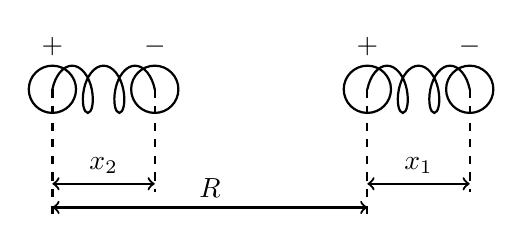
\begin{tikzpicture}[thick]
            \usetikzlibrary{decorations.pathmorphing,calc}
            \draw[decorate,decoration={coil,aspect=0.5,amplitude=3mm,segment length=4mm}] (0,0) -- (1.3,0);
            \draw (0,0) circle (3mm) node[above=3mm]{\(+\)};
            \draw (1.3,0) circle (3mm) node[above=3mm]{\(-\)};
            \draw[dashed] (0,0) -- ++(0,-1.6);
            \draw[dashed] (1.3,0) -- ++(0,-1.3);
            \draw[<->] (0,-1.2) -- node[above]{\(x_2\)} (1.3,-1.2);
            \draw[decorate,decoration={coil,aspect=0.5,amplitude=3mm,segment length=4mm}] (4,0) -- (5.3,0);
            \draw (4,0) circle (3mm) node[above=3mm]{\(+\)};
            \draw (5.3,0) circle (3mm) node[above=3mm]{\(-\)};
            \draw[dashed] (4,0) -- ++(0,-1.6);
            \draw[dashed] (5.3,0) -- ++(0,-1.3);
            \draw[<->] (4,-1.2) -- node[above]{\(x_1\)} (5.3,-1.2);
            \draw[<->] (0,-1.5) -- node[above]{\(R\)} (4,-1.5);
        \end{tikzpicture}
    \end{center}
    \begin{enumerate}[label=(\alph*)]
        \item Seja \(P_1\) e \(P_2\) os operadores de momento linear de cada um dos átomos oscilantes. Escreva o hamiltoniano \(H_0\) do sistema de dois osciladores harmônicos sem carga, logo sem interação entre eles.
        \item Escreva o hamiltoniano \(H_1\) que representa a energia de acoplamento (energia eletrostática) entre os dois osciladores carregados.
        \item Na aproximação de pequenas oscilações \(x_1, x_2 \ll R\), encontre \(H_1\) em ordem mais baixa do desenvolvimento em série.
        \item Usando a aproximação para \(H_1\) encontrada no item (c), determine a expressão para o hamiltoniano \(H = H_0 + H_1\) usando as seguintes transformações
            \begin{align*}
                x_1 &= \frac{1}{\sqrt{2}} (x_s + x_a) &
                x_2 &= \frac{1}{\sqrt{2}} (x_s - x_a)\\
                P_1 &= \frac{1}{\sqrt{2}} (P_s + P_a) &
                P_2 &= \frac{1}{\sqrt{2}} (P_s - P_a).
            \end{align*}
        \item Determine as frequências de oscilação de cada um dos osciladores acoplados e calcule, em segunda ordem (até \(R^{-6}\)), uma aproximação para cada uma dessas frequências.
        \item Determine a energia de interação entre os osciladores no seu estado fundamental.
    \end{enumerate}
\end{exercício}
\begin{proof}[Resolução]
    Sem interação entre os osciladores harmônicos, temos
    \begin{equation*}
        H_0 = \frac{1}{2m}(P_1^2 + P_2^2) + \frac{1}{2}m \omega^2 (x_1^2 + x_2^2).
    \end{equation*}
    O acoplamento entre os osciladores harmônicos é dado pelo hamiltoniano
    \begin{equation*}
        H_1 = \frac{e^2}{R} + \frac{e^2}{R + x_1 - x_2} - \frac{e^2}{R+x_1} - \frac{e^2}{R - x_2},
    \end{equation*}
    onde definimos \(e^2 = \frac{q^2}{4\pi \epsilon_0}\). Notemos que
    \begin{align*}
        H_1 &= \frac{e^2}{R} + \frac{e^2}{R}\left(1 + \frac{x_1 - x_2}{R}\right)^{-1} - \frac{e^2}{R} \left(1 + \frac{x_1}{R}\right)^{-1} - \frac{e^2}{R}\left(1 - \frac{x_2}{R}\right)^{-1} \\
            &= \frac{e^2}{R}\left[1 + \left(1 + \frac{x_1 - x_2}{R}\right)^{-1} - \left(1 + \frac{x_1}{R}\right)^{-1} - \left(1 - \frac{x_2}{R}\right)^{-1}\right],
    \end{align*}
    portanto
    \begin{align*}
        \diffp{H_1}{x_1} &= \frac{e^2}{R^2}\left[\left(1 + \frac{x_1}{R}\right)^{-2} - \left(1 + \frac{x_1 - x_2}{R}\right)^{-2}\right]&
        \diffp{H_1}{x_2} &= \frac{e^2}{R^2}\left[\left(1 + \frac{x_1 - x_2}{R}\right)^{-2} - \left(1 - \frac{x_2}{R}\right)^{-2}\right]\\
        \diffp[2]{H_1}{x_1} &= -\frac{2e^2}{R^3}\left[\left(1 + \frac{x_1}{R}\right)^{-3} - \left(1 + \frac{x_1 - x_2}{R}\right)^{-3}\right]&
        \diffp[2]{H_1}{x_2} &= \frac{2e^2}{R^2}\left[\left(1 + \frac{x_1 - x_2}{R}\right)^{-3} - \left(1 - \frac{x_2}{R}\right)^{-3}\right]
    \end{align*}
    e
    \begin{equation*}
        \diffp{H_1}{x_1,x_2} = \diffp{H_1}{x_2,x_1} = -\frac{2e^2}{R^3}\left(1 + \frac{x_1 - x_2}{R}\right).
    \end{equation*}
    Avaliando em \((x_1,x_2) = (0,0)\), temos verificamos que todos os temos se anulam, exceto pela derivada mista, que é negativa, portanto este ponto é um ponto de equilíbrio estável e podemos aproximar
    \begin{equation*}
        H_1 \simeq \diffp{H_1}{x_1,x_2}[(0,0)]x_1x_2 = -\frac{2e^2x_1x_2}{R^3}
    \end{equation*}
    para \(x_1,x_2 \ll R\). Neste limite, o hamiltoniano do sistema é dado por
    \begin{align*}
        H &= \frac{1}{2m}(P_1^2 + P_2^2) + \frac12 m \omega^2(x_1^2 + x_2^2) - \frac{2e^2x_1x_2}{R^3}\\
          &= \frac{(P_s + P_a)^2 + (P_s - P_a)^2}{4m} + \frac{m \omega^2\left[(x_s + x_a)^2 + (x_s - x_a)^2\right]}4  -\frac{e^2(x_s^2 - x_a^2)}{R^3}\\
          &= \frac{P_s^2 + P_a^2}{2m} + \frac{m \omega^2\left[x_s^2 + x_a^2\right]}2  -\frac{e^2(x_s^2 - x_a^2)}{R^3}\\
          &= \frac{P_s^2}{2m} + \frac12m\left(\omega^2 - \frac{e^2}{mR^3}\right)x_s^2 + \frac{P_a^2}{2m} + \frac12 m\left(\omega^2 + \frac{e^2}{m R^3}\right)x_a^2,
    \end{align*}
    portanto as frequência dos modos normais são dadas por
    \begin{equation*}
        \omega_s^2 = \omega^2 - \frac{e^2}{mR^3}\quad\text{e}\quad\omega_a^2 = \omega^2 + \frac{e^2}{m R^3}.
    \end{equation*}
\end{proof}
